%++++++++++++++++++++++++++++++++++++++++
% Don't modify this section unless you know what you're doing!
\documentclass[letterpaper,12pt]{article}
\usepackage{tabularx} % extra features for tabular environment
\usepackage{amsmath}  % improve math presentation
\usepackage{graphicx} % takes care of graphic including machinery
\usepackage[margin=1in,letterpaper]{geometry} % decreases margins
\usepackage{cite} % takes care of citations
\usepackage[final]{hyperref} % adds hyper links inside the generated pdf file
\hypersetup{
	colorlinks=true,       % false: boxed links; true: colored links
	linkcolor=blue,        % color of internal links
	citecolor=blue,        % color of links to bibliography
	filecolor=magenta,     % color of file links
	urlcolor=blue         
}
%++++++++++++++++++++++++++++++++++++++++


\begin{document}

\title{COMP 512 Phase 1 Report}
\author{Yiwei Xia and Marie Payne}
\date{\today}
\maketitle

\section{Introduction}

The goal of our project is to design and develop a distributed system where clients can make requests and servers deliver responses based upon them, with the use of a middleware server. The aim is to develop this system using two protocols, remote method invocation and through transmission control protocol (TCP).

\section{Theory}

// some theory about RMI
// some theory about TCP
// use figures included in github to demonstrate points, cite them to Tanenbaum's textbook on distributed systems (more citation info in slides)


\begin{figure}[ht] 
	% read manual to see what [ht] means and for other possible options
	\centering 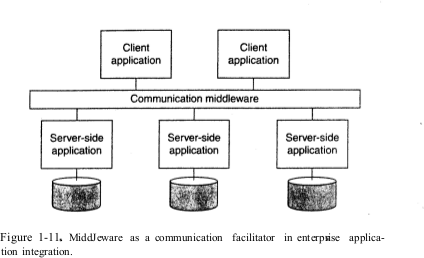
\includegraphics[width=0.8\columnwidth]{figure1.png}
	% note that in above figure file name, "sr_setup",
	% the file extension is missing. LaTeX is smart enough to find
	% apropriate one (i.e. pdf, png, etc.)
	% You can add this extention yourself as it seen below
	% both notations are correct but above has more flexibility
	%\includegraphics[width=1.0\columnwidth]{sr_setup.pdf}
	\caption{
		\label{fig:samplesetup} % spaces are big no-no withing labels
		% things like fig: are optional in the label but it helps
		% to orient yourself when you have multiple figures,
		% equations and tables
		Every figure MUST have a caption.
	}
\end{figure}


\begin{figure}[ht] 
	% read manual to see what [ht] means and for other possible options
	\centering 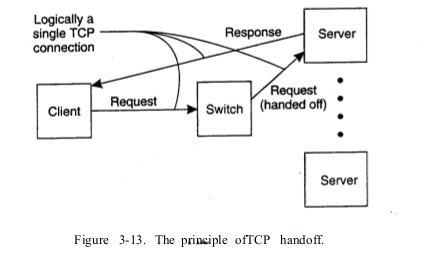
\includegraphics[width=0.8\columnwidth]{figure2.png}
	% note that in above figure file name, "sr_setup",
	% the file extension is missing. LaTeX is smart enough to find
	% apropriate one (i.e. pdf, png, etc.)
	% You can add this extention yourself as it seen below
	% both notations are correct but above has more flexibility
	%\includegraphics[width=1.0\columnwidth]{sr_setup.pdf}
	\caption{
		\label{fig:samplesetup} % spaces are big no-no withing labels
		% things like fig: are optional in the label but it helps
		% to orient yourself when you have multiple figures,
		% equations and tables
		Every figure MUST have a caption.
	}
\end{figure}



\section{Design}

// a few lines about the rmi middleware
// a few lines about the tcp middleware
// 'testing' we did (lol) 

\section{Conclusion}

Distributing the servers and server requests is a very efficient way to model client-server architecture. The use of the middleware server facilitates this process and provides concurrency to the system. 

\end{document}